\subsection{Why exocentric vision ?}
\frame
{
  \frametitle{Why exocentric vision ?}
  
  \emph{It's difficult for an operator not accustomed to the vehicle
    to estimate the vehicle's position and direction and the distances to a target, strictly
    based on camera images from the first person viewpoint\footnote{\tiny{as stated by M. Sugimoto and others}}.}
  \pause
  
  \vskip15pt

  \begin{block} {\alert{\texttt{Idea}}}
    An exocentric camera would provide a view of the robot in the operating
    environment and, thus, a better understanding of where the robot is located into the
    environment and its actual direction.
  \end{block}
  
  \pause
    
  \vskip5pt
  
  \begin{block} {\alert{\texttt{Trouble}}}
    Exocentric camera could be mounted on a rear-mounted protuberance of the robot,
    but such a protuberance would terribly limit the robot activity and its moving abilities.
  \end{block}
  
}

\frame
{
  \frametitle{Why exocentric vision ?}

  \begin{block} {\alert{\texttt{Solution}}}
    Simulate a virtual \textbf{exocentric} point of view, by drawing with augmented reality
    the robot on previous recorded first-person (i.e. \textbf{egocentric}) images, shot along its path. \\
    \pause
    Set a previous image as \textbf{texture}, robot is virtually drawn in order to
    simulate what a \textbf{rear} camera would shoot.  
  \end{block}

  %\vskip8pt
  \pause
  
  \begin{columns}
    
    \column{0.4\textwidth}
    \visible<3-> {
      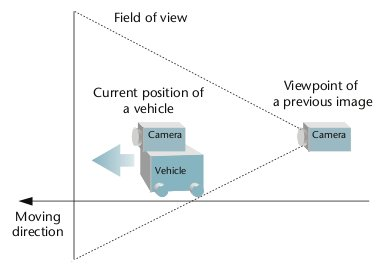
\includegraphics[width=\textwidth]{img/exocentric_vision.jpg}
    }

    \pause
    
    \column{0.2\textwidth}
    \visible<4-> {
      \begin{center}
        $\Longrightarrow$ \\
        \alert{virtual exocentric}
        \vskip4pt
        \scriptsize{with augmented reality}
      \end{center}
    }

    \pause

    \column{0.4\textwidth}
    \visible<5-> {
      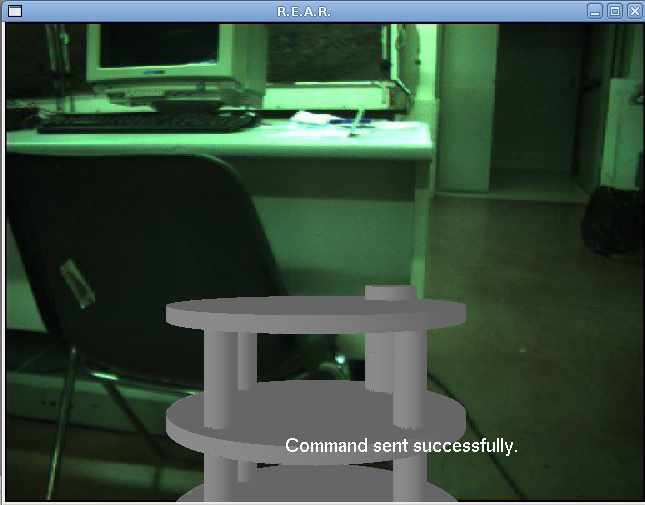
\includegraphics[width=\textwidth]{img/virtual_exocentric.png}
    }
    
  \end{columns}
  
  \pause
  
  \begin{block} {\alert{\texttt{Drawback}}}
    Environment must not change frequently.
  \end{block}


}

\subsection{Main issues}
\frame
{
  \frametitle{Main issues}


  
  \begin{block} {\alert{\texttt{We need to determinate}}}
    
    \pause
    
    \begin{itemize}
      
    \item \alert{\textit{how to draw the robot}} \\
      different robots must be drawn accordingly to
      their physical characteristics
      \pause
      
    \item \alert{\textit{how to choose the best image}} \\
      among all the egocentric images collected, we need
      the one able to provide the \textbf{most
      comprehensible} external robot view
      \pause
      
    \item \alert{\textit{how to place the robot}} \\
      where to overlap a 3D robot representation
      in virtual space
    \end{itemize}
    
  \end{block}
}
